\documentclass[a4paper,12pt,dutch]{article}
\usepackage{glossaries}
\usepackage[T1]{fontenc}
\usepackage{babel}
\usepackage{graphicx}
\usepackage[table,xcdraw]{xcolor}
\usepackage{hyperref}
\usepackage{blindtext}
\usepackage{geometry}
\usepackage{parskip}
\usepackage{mathtools}
\usepackage{siunitx}
\usepackage{listings}
\usepackage{csquotes}
\usepackage{caption}
\usepackage{subcaption}
\usepackage{comment}
\usepackage{pdfpages}
\usepackage[useregional]{datetime2}
\usepackage{amsmath} % for the equation* environment
\usepackage{float}
\usepackage{pict2e}
\usepackage{fixltx2e}

\DeclareRobustCommand{\slashcirc}{{\mathpalette\doslashcirc\relax}}

\makeatletter
\newcommand\doslashcirc[2]{%
  \sbox\z@{$#1\m@th\circ$}%
  \setlength\unitlength{\wd\z@}
  \begin{picture}(1,1)
  \roundcap
  \put(0,0){\box\z@}
  \put(0,0){\line(1,1){1}}
  \end{picture}%
}
\makeatother


% %% Some packages you will need
% \usepackage{pgfplots}
% \usepackage{pgfplotstable}
% \usepackage{booktabs}
% \usepackage{array}
% \usepackage{colortbl}


\definecolor{arduinoorange}{HTML}{FFA500}
\definecolor{arduinogray}{HTML}{808080}
\definecolor{arduinoblue}{HTML}{007ACC}
\definecolor{arduinogreen}{HTML}{469B00}

\lstset{
  language=C++,
  basicstyle=\ttfamily\footnotesize,
  keywordstyle=\color{arduinoorange},
  stringstyle=\color{arduinogreen},
  commentstyle=\color{arduinogray},
  moredelim=[s][\color{arduinoblue}]{\#}{\ },
  morekeywords={digitalRead,digitalWrite,pinMode,analogRead,analogWrite,Serial,begin,HIGH,LOW},
  frame=tb,
  tabsize=4,
  showstringspaces=false,
  breaklines=true,
  numbers=left,
  numberstyle=\tiny\color{arduinogray},
  numbersep=5pt,
  extendedchars=true,
  literate={á}{{\'a}}1 {ã}{{\~a}}1 {é}{{\'e}}1,
}

\lstdefinestyle{Arduino}
{
  language=C++,
  basicstyle=\ttfamily\footnotesize,
  keywordstyle=\color{arduinoorange},
  stringstyle=\color{arduinogreen},
  commentstyle=\color{arduinogray},
  moredelim=[s][\color{arduinoblue}]{\#}{\ },
  morekeywords={digitalRead,digitalWrite,pinMode,analogRead,analogWrite,Serial,begin},
  frame=tb,
  tabsize=4,
  showstringspaces=false,
  breaklines=true,
  numbers=left,
  numberstyle=\tiny\color{arduinogray},
  numbersep=5pt,
  extendedchars=true,
  literate={á}{{\'a}}1 {ã}{{\~a}}1 {é}{{\'e}}1,
  backgroundcolor=\color{black!85},
  rulecolor=\color{arduinoorange},
  frame=single,
  frameround=tttt,
  framexleftmargin=6pt,
  framexrightmargin=6pt,
  framextopmargin=6pt,
  framexbottommargin=6pt,
  breaklines=true,
  postbreak=\raisebox{0ex}[0ex][0ex]{\ensuremath{\color{red}\hookrightarrow\space}},
}

\usepackage[
    backend=biber,
    backref=true,
    backrefstyle=none,
    sortcites=true,
    sorting=none,
    doi=false, % doi informatie wordt niet weergegeven
    %uniquename=true,
    %uniquelist=true,
    maxcitenames=3,
    %issn=false, werkt niet
    language=american
]{biblatex}
\addbibresource{information/Bronnen.bib}
\DefineBibliographyStrings{dutch}{
    backrefpage = {blz.},
    backrefpages = {blz.},
}
\makeglossaries
\definecolor{Grey1}{HTML}{343434}
\graphicspath{{./Media/Figuren/}}
 \geometry{
 a4paper,
 total={170mm,257mm},
 left=20mm,
 top=20mm,
 }
\hypersetup{
    colorlinks=true,
    linkcolor=blue,
    filecolor=magenta,      
    urlcolor=cyan,
    pdftitle={Overleaf Example},
    pdfpagemode=FullScreen,
    }


\begin{document}
\title{

\includegraphics[width=3.5in]{IMG/logo/finalcircle.png} \\
\vspace*{1in}
\textbf{Project 3}\\
\textit{PVA Duurzame Energie}\\
Versie 1
}
\author{
\vspace*{1in} \\
  Geschreven door:\\
  Laurens van der Drift\\
  Tommy Dobos\\
		\vspace*{0.2in} \\
		De Haagse Hogeschool\\
        \textbf{Elektrotechniek}\\
        Delft, Nederland
       } 
\maketitle
\phantomsection
\section*{Versie Historie} \addcontentsline{toc}{section}{Versie Historie}

\begin{table}[h]
\begin{tabular}{|l|l|l|l|}
\hline
\rowcolor[HTML]{4472C4} 
{\color[HTML]{FFFFFF} \textbf{Versie}} &
  {\color[HTML]{FFFFFF} \textbf{Datum}} &
  {\color[HTML]{FFFFFF} \textbf{Wijzigingen}} &
  {\color[HTML]{FFFFFF} \textbf{Auteur}} \\ \hline
\rowcolor[HTML]{D9E1F2} 
1.0 &
  \multicolumn{1}{c|}{\cellcolor[HTML]{D9E1F2}\date{\today}} &
 N.v.t. &
  Cleaneco \\ \hline

% \rowcolor[HTML]{FFFFFF} 
% 2.0 &
%   \multicolumn{1}{c|}{\cellcolor[HTML]{FFFFFF}7-4-2023} &
%  Feedback van FeedbackFruits toegepast &
%   Infra   Vroom \\ \hline

% \rowcolor[HTML]{D9E1F2} 
% 3.0 &
%   \multicolumn{1}{c|}{\cellcolor[HTML]{D9E1F2}4-6-2023} &
%  Bijgewerkt voor Assessment 3 &
%   Infra   Vroom \\ \hline

\end{tabular}
\end{table}
%\addcontentsline{toc}{section}{Verklarende Woordenlijst}
\printglossaries
\newglossaryentry{tender}
{
    name=\textit{tender},
    description={De inschrijving om op een kavel een wind turbine park te bouwen.}
}
\newglossaryentry{energie akkoord}
{
    name=\textit{energie akkoord},
    description={Het Energieakkoord vertegenwoordigt duurzame groei, met betrokkenheid van 40+ organisaties waaronder overheid, werkgevers en milieuactivisten. Het bevat afspraken over energiebesparing, schonere technologie en klimaatbeleid.}
}
\newglossaryentry{offshore}
{
    name=\textit{offshore},
    description={Op enige afstand van de kust.}
}
\newglossaryentry{subsidie}
{
    name=\textit{subsidie},
    description={Een financiële bijdrage die je kunt krijgen van een overheids- of een particuliere organisatie.}
}
\newglossaryentry{joint venture}
{
    name=\textit{joint venture},
    description={Een joint venture (gezamenlijke onderneming) is een afspraak tussen bestaande bedrijven om samen te werken.}
}
\newglossaryentry{natuurinclusief}
{
    name=\textit{natuurinclusief},
    description={Natuurinclusief bouwen betekent dat er bewust ruimte voor biodiversiteit wordt gecreëerd op, aan of in het gebouw of de (openbare) omgeving, zodat er meer diverse planten- en diersoorten kunnen leven.}
}
\phantomsection
\addcontentsline{toc}{section}{Lijst van figuren}
\listoffigures
\newpage
\tableofcontents
% \section{Voorwoord}
Cleaneco is een bedrijf ontstaan in augustus 2023 te Delft en is opgericht door Laurens van der Drift en Tommy Dobos.

Ingenieurs- en consultancybureau Worley heeft het ontwerp bedrijf Cleaneco aangenomen om een offshore windpark te ontwerpen op kavel VI en VII van Hollandse Kust West en hiervoor de tender te schrijven voor Rijkswaterstaat. 

De reden voor de aanleg van het windturbinepark op zee is hoofdstuk 4.2.2 van het energie akkoord\cite{energieakkoord} van 6 september 2013. In dit akkoord is afgesproken dat in 2023, 4450MW aan windvermogen op zee opgewekt moet worden. Met als doel genoeg vermogen opwekken voor vijf miljoen huishoudens. 

% \section{Samenvatting}
\subsection{Project naam}
Voor dit project, Project Windpark Op Zee is het bedrijf Cleaneco in dienst genomen door Worley. 

\subsection{Probleem}
De Nederlandse overheid moet voldoen aan het \gls{energie akkoord}\cite{energieakkoord}, dat is vastgelegd op 6 september 2013. Dit akkoord stelt dat tegen 2023 een uitbreiding van het operationeel windvermogen op zee moet zijn gerealiseerd van 3450 MW. De al bestaande parken wekken ongeveer 1000 MW op. Samen zal dit dus ongeveer 4450 MW aan windvermogen moeten worden.

% De Nederlandse overheid moet voldoen aan het \gls{energie akkoord} vastgelegd op 6 september 2013.
% Hierin staat aangegeven dat in 2023 een opschaling moet hebben plaatsgevonden voor een operationeel windvermogen op zee van 4450MW. De reeds bestaande parken en hetgeen reeds in de pijplijn zit, tellen op tot circa 1000MW.
% Hoe kan de Nederlandse overheid de groei van windenergie op zee naar 4450 MW operationeel vermogen in 2023 bevorderen, met focus op kostenreductie, technologische vooruitgang, ruimtelijke planning en het overwinnen van belemmeringen, om zo aan de eisen te voldoen van het \gls{energie akkoord} opgesteld in september 2023?

\subsection{Doelstelling en Resultaat}
Onder opdracht van Worley is het aan Cleaneco om een technisch ontwerp te maken van een windturbinepark op zee. Hiervoor moet ook een onderhoudsplan worden opgesteld voor de komende 25 jaar. Het technisch ontwerp en onderhoudsplan zullen in de vorm van een adviesrapport aan de opdrachtgever gepresenteerd worden.

Uiterlijk in 2023 wordt een operationeel windvermogen van 4450 MW op zee gerealiseerd, in overeenkomst met de eisen van het \gls{energie akkoord}\cite{energieakkoord} van september 2013. Dit wordt bereikt met meetbare kostenverlaging, technologische vooruitgang, doelgerichte ruimtelijke planning en het succesvol aanpakken van belemmeringen. Dit project heeft significante maatschappelijke relevantie, het draagt namelijk bij aan de verduurzaming van de energieopwekking. Naast de naar schatting vijf miljoen\cite{energieakkoord} huishoudens die zullen profiteren van de duurzame energievoorziening, zal dit project bijdragen aan het vergroten van de kennis en ervaring op het front van windparken op zee.  

\subsection{Eisen} \label{Eisen}
Er moet aan de volgende eisen worden voldaan:
\begin{itemize}
   \item Er moet onderzoek gedaan worden naar nodige producten/materialen zoals: windturbines, kabels en transformator boxen. Hierbij moeten de energieopbrengsten voor twee verschillende turbines worden onderzocht.
   \item Er moeten twee verschillende ontwerpen komen voor de positionering van de windturbines. 
   \item Er moet een operationeel windvermogen op zee van 4450MW opgeleverd worden.
   \item Er moet een onderhoudsplan meegeleverd worden voor de komende 25 jaar.
   % \item Alles moet in een adviesrapport aan de opdrachtgever Worley gepresenteerd worden. 
   \item Alles moet in een adviesrapport gepresenteerd worden aan de opdrachtgever Worley.
 \end{itemize}

\subsection{Probleem oplossing}
Cleaneco zal een ontwerprapport en onderhoudsplan leveren aan Worley. Het rapport beantwoordt de \gls{tender} voor het \gls{offshore} windturbinepark. Het onderhoudsplan waarborgt dat het \gls{offshore} windpark op zee 25 jaar operationeel is. Bij projectvoltooiing volgt een adviesrapport. Om dit te realiseren zal onderzoek gedaan worden naar de punten genoemd onder hoofdstuk \ref{Eisen}. 

Het type onderzoek zal vallen onder het zogenoemde, bronnenonderzoek. De bronnen zullen onder andere komen van de database van de Haagse Hogeschool en professionals in het betreffende vakgebied.

% % \section{Kosten en Opbrengsten}
%     \subsection{Financiële kosten en budget}
%     Bouwkosten Windpark: Hoewel specifieke bouwkosten niet worden vermeld in de verstrekte informatie, kan worden aangenomen dat de bouw van een windpark van 756 MW met 54 windturbines aanzienlijke kapitaalinvesteringen met zich meebrengt. Dit omvat de kosten voor het ontwerpen, fabriceren en installeren van de windturbines en de benodigde infrastructuur op zee.

%     Milieueffectrapportages en Locatiestudies: Er wordt vermeld dat Ecowende kosten draagt voor milieueffectrapportages en locatiestudies. Deze studies zijn nodig om de impact van het windpark op het milieu en de omgeving te beoordelen en te minimaliseren.

%     Overheidsinkomsten: De overheid ontvangt € 63,5 miljoen van de partijen als gevolg van financiële biedingen en bijdragen van Ecowende. Dit geld wordt gebruikt om nieuwe windparken beter te integreren in de omgeving en voor overige activiteiten op de Noordzee.

%     % \subsection{Verklarende woordenlijst}
% Tijdslijn van het Project:

%     2022: Ecowende, een \gls{joint venture} van Shell en Eneco, wint de vergunning voor het windpark Hollandse Kust (west) kavel VI.

%     2023: Ontwerp en plannen worden gemaakt, en de bouw van het windpark is gepland om te beginnen in dit jaar.

%     2026: Het windpark wordt naar verwachting volledig operationeel en levert elektriciteit.

% Het maken van het windturbineparkontwerp en het onderhoudsplan zal gebeuren in een periode van 17 weken. Hiervan zal aan het begin ongeveer 60\% van de tijd besteed worden aan het maken van het windparkontwerp, de overige tijd zal worden gestoken in het realiseren van het onderhoudsplan en het verwerken van beide producten in het adviesrapport.\cite{studiewijzer} 

% \subsection{Opbrengsten}

%     Duurzame Energievoorziening: Het windpark Hollandse Kust (west) zal naar verwachting een vermogen van 756 MW genereren. Dit komt overeen met ongeveer 3\% van de Nederlandse elektriciteitsvraag, wat voldoende is om ongeveer een miljoen huishoudens van elektriciteit te voorzien. De opbrengst voor eindgebruikers is een toename van duurzame energievoorziening en een verminderde afhankelijkheid van niet-hernieuwbare bronnen zoals fossiele brandstoffen.

%     Milieubescherming: Het ontwerp van het windpark is '\gls{natuurinclusief}' en omvat maatregelen om de impact op de natuur en het milieu te minimaliseren. Dit omvat bijvoorbeeld het creëren van een gezond ecosysteem, het minimaliseren van de impact op vogels, het onderwaterleven, en het stimuleren van biodiversiteit onder water. De opbrengst hier is een stap in de richting van milieubescherming en behoud van biodiversiteit.

%     Toekomstige Groene Energie: Het windpark maakt deel uit van de groeiende inspanningen om groene energie in Nederland te vergroten. Dit draagt bij aan de ambitie om tegen 2030 ongeveer 21 GW aan windenergie op zee te hebben, wat een duurzame energiebron voor de toekomst zal opleveren.

%     Economische Impuls: De bouw van windparken op zee kan een economische impuls geven aan de regio, met potentiële werkgelegenheidskansen in havens zoals Vlissingen, IJmuiden, Den Helder en de Eemshaven.

% Samengevat, het project levert duurzame energie, milieubescherming, toekomstige groene energiebronnen en economische kansen op voor de eindgebruikers en de samenleving als geheel.\cite{Windenergiegebied}\cite{ShellEneco}\cite{Windopzee}

% % Opbrengst:

% % https://www.noordzeeloket.nl/functies-gebruik/windenergie/doorvaart-medegebruik/hollandse-kust-west/

% % https://www.rvo.nl/onderwerpen/bureau-energieprojecten/afgesloten-projecten/woz-hollandse-kust-west-kavels-vi-vii

% % https://www.rijksoverheid.nl/actueel/nieuws/2022/12/15/shell-en-eneco-winnen-tender-windpark-op-zee-hollandse-kust-west
% \section{Opdracht analyse}


% \section{Projectgrenzen}
% \subsection{Wat wel}
% \begin{itemize}
%     \item Wij schrijven een plan van aanpak.
%     \item Wij doen onderzoek naar de technische aspecten en de energie opbrengsten.
%     \item Wjj doen onderzoek naar de verschillende windturbines, transformatoren, bekabeling en toebehoren.
%     \item Wij schrijven een onderhoudsplan voor 25 jaar waarbij we gebruik maken van levensduur en statistische gegevens.
%     \item Wij maken een parkontwerp waarbij rekening wordt gehouden met een optimale plaatsing van de windturbines.
%     \item Wij presenteren ons parkontwerp en onderhoudsplan aan onze opdrachtgever: Worley.
% \end{itemize}
% \subsection{Wat niet}
% \begin{itemize}
%     \item Wij vragen geen vergunning aan voor een \gls{offshore} windpark op zee.
%     \item Wij vragen geen subsidie aan bij de Nederlandse overheid.
%     \item Wij beheren geen elektrische infrastructuur (wordt gedaan door TenneT\cite{energieakkoord}).
%     \item Wij realiseren geen \gls{offshore} windpark op zee.
%     \item Wij zijn niet verantwoordelijk voor oplopende problemen tijdens de realisatie fase van het \gls{offshore} windpark op zee.
% \end{itemize}
% \subsection{Verwachte tijdsduur}
% Op dinsdag 29 augustus zijn we begonnen aan het project \textit{Duurzame Energie} en we plannen om hier 17 weken aan te besteden. In week 19 staat onze eindpresentatie gepland voor onze opdrachtgever Worley, die zal plaatsvinden op hun kantoor in Den Haag. 
% We schatten in dat we gedurende dit project ongeveer 16 x 2 contacturen en 16 x 6 zelfstudie-uren zullen besteden\cite{studiewijzer}.


% \section{Programma van eisen}
\subsection{Plan van Aanpak}
Het eerste product dat geleverd zal worden is het plan van aanpak. In het plan van aanpak staan alle plannen en belangrijke informatie voor het opzetten van het project. Dit document zal worden geleverd voordat aan het project begonnen wordt. Daarnaast zal het ook gepresenteerd worden in een korte pitch van twee minuten. Het doel van het plan van aanpak is, het creëren van duidelijkheid over: de verwachtingen van de opdrachtgever, de doelen waar naartoe moet worden gewerkt en hoe, en de belangrijke informatie over het project, zoals mogelijke risico's, te ondernemen acties en de werkwijze. 

\subsection{Parkontwerp}
Het tweede product dat gemaakt en geleverd zal moeten worden is het parkontwerp. Het windturbinepark staat in dit project centraal, hiervan zal dan ook een uitgewerkt ontwerp worden geleverd. Hierin worden technische aspecten behandeld, zo zullen twee type windturbines worden uitgewerkt, voor beide zal ook de optimale positionering worden bepaald voor de beste opbrengst. Dit zal bepaald worden door het gedrag van de wind op de kavels te analyseren. Er zal ook worden ingegaan op de verwachte energieopbrengsten voor de gekozen turbines. 

Bij het parkontwerp hoort natuurlijk ook een uitwerking van de bekabeling, de specificaties van de kabels zelf, en de uitwerking van de onderlinge connecties en die met het hoogspanningsstation. Bij het ontwerpen van het windturbinepark zal ook rekening worden gehouden met het effect dat alle hiervoor genoemde elementen zullen hebben op de onderhoud van het park. 

\subsection{Onderhoudsplan}
Het derde product dat geleverd zal worden is het onderhoudsplan. In het onderhoudsplan zal komen welke componenten, met welke frequentie, onderhoud nodig zullen hebben. Ook wordt ingegaan op de soort onderhoud en hoe dit moet gebeuren. De frequentie zal worden gebaseerd op en onderbouwd door statistische gegevens over de verschillende componenten van windturbineparken. Met de frequentie zal vervolgens een onderhoudsstrategie gemaakt worden dat ook verwerkt wordt in het onderhoudsplan. 

Verder zal er in het onderhoudsplan worden besproken hoe de conditie van de componenten bewaakt zal worden. Ten slotte zullen de risico's van het plegen van onderhoud worden uitgewerkt in het plan. 

\subsection{Adviesrapport}
Als laatste product zal het adviesrapport worden opgesteld voor Worley. In het adviesrapport zullen de belangrijkste aspecten van de vorige producten worden samengevat. Zo zal de probleemstelling van het project aan bod komen samen met de gekozen turbine types en verwachte energieopbrengsten. Verder zal het parkontwerp inclusief bekabeling en de bijbehorende kabelberekeningen in het adviesrapport worden verwerkt. Ten slotte zal ook het onderhoudsplan niet uit het adviesrapport worden weggelaten. Ter afsluiting van het project zal dit adviesrapport (aan Worley) worden gepresenteerd. 

% Onpersoonlijk:
\section{Wat zijn de belangrijke aspecten van de kavels VI en VII?} \label{Wat zijn de belangrijke aspecten van de Kavels VI en VII?}

Er zijn veel aspecten van de kavels VI en VII waar rekening mee moet worden gehouden. Enkele belangrijker dan anderen. Ten eerste is de locatie van de kavels van belang. De kavels maken onderdeel uit van het windenergiegebied Hollandse Kust west en liggen op ongeveer 53 km van de west kust van Nederland en heeft een oppervlakte van circa 176 km\textsuperscript{2}.\cite{SiteDescriptionRVO} De twee kavels zullen elk een \gls{offshore} windcapaciteit van 700MW realiseren.\cite{SiteDescriptionRVO}\cite{Functies&gebruikHKW}

Om het windpark te ontwerpen dat instaat is dit te bieden zijn verschillende andere data van de kavels belangrijk. Er moet bepaald worden wat de beste positionering is voor de windturbines. Bij de beslissing hiervan moeten aspecten in acht genomen worden, zoals al bestaande en geplande infrastructuur van pijpleidingen en kabels. Daarnaast moet rekening worden gehouden met potentiële wrakken, magnetische abnormaliteiten en oude boorgaten zoals genoteerd staat in Appendix C van de locatie beschrijving (zie figuur \ref{fig:obstakels}).\cite{SiteDescriptionRVO}\cite{AppendixC} Uit voorzorg zullen, de windturbines op een minimale afstand van 100 meter van de genoemde obstakels geplaatst worden. Dit zal echter pas later van toepassing zijn, aangezien er voorlopig nog geen parkindeling is gemaakt. 
\begin{figure}[h]
\centering
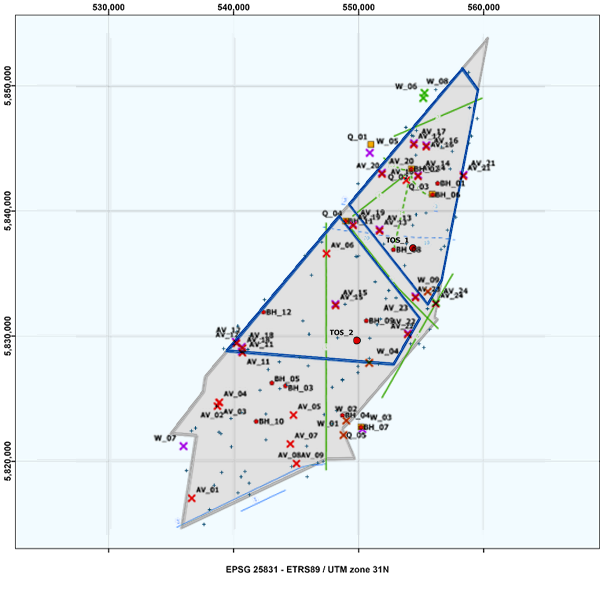
\includegraphics[width=0.5\textwidth]{IMG/data/overzicht/Map.png}
\caption{Gecombineerde map van obstakels.}
\label{fig:obstakels}
\end{figure}

Er is ook informatie over de kavels die significant is voor het besluit over de te kiezen windturbines en de oriëntatie hiervan. De informatie die hiervoor belangrijk is, is de winddata, zoals windsnelheden en -richtingen over langere periodes. Deze data is te halen uit de Wind Resource Assessment.\cite{WindResourceAssessment} In dit document staat winddata van metingen die zijn uitgevoerd over een periode van twee jaar, van 07-02-2019 tot 06-02-2021. Deze metingen zijn gedaan op een hoogte van 100 meter boven het gemiddelde zeeniveau en zijn dus representatief voor de te verwachten winden die de windturbines zullen ervaren. De statisch gemiddelde gemeten windsnelheid was over deze periode 10,06 m/s. 

Behalve de windsnelheid, is ook de windrichting van belang. De windrichting was net zoals de windsnelheid variërend, echter is er wel een overheersende windrichting bepaald. De overheersende windrichting is WZW (West-Zuid-West), deze windrichting kwam voor 21,2\% van de gemeten periode voor. De tweede meest significante windrichting was ZZW (Zuid-Zuid-West), met 20,1\%. 





% Er is naar een veelvoud windturbines gezocht en gekeken. Bekeken modellen waren onder andere de volgende:
% \begin{itemize}
%     \item De SG 14-236 DD, 14 MW windturbine van Siemens Gamesa.\cite{SiemensGamesa14MW}
%     \item De V236-15.0, 15 MW windturbine van Vestas.
%     \item De Haliade-X, 12 MW windturbine van GE renewable energy.\cite{GEHalideX}
%     \item 
% \end{itemize}

\section{Berekeningen}
\subsection{Algemene berekeningen}
\subsubsection{Swept Area}
Van de uitgekozen windturbines zijn meerdere gegevens verzameld, waaronder de diameter. Hiermee is het rotoroppervlakte (A(\(m^2\))) te berekenen zoals gedaan in formules \ref{eq:1} en \ref{eq:2}.
\begin{equation} \label{eq:1}
% \text{12MW Turbine geeft: } \pi*(\slashcirc/2)^2 = \pi*(222/2)^2 = 38707
\text{12MW Turbine geeft: } A =\pi*(\frac{\slashcirc_{12MW}}{2})^2 = \pi*(\frac{222}{2})^2 = 38707 m^2
\end{equation}
\myequations{Berekening: A 12MW Turbine}

\begin{equation} \label{eq:2}
\text{18MW Turbine geeft: } A =\pi*(\frac{\slashcirc_{18MW}}{2})^2 = \pi*(\frac{263}{2})^2 = 54325 m^2
\end{equation}
\myequations{Berekening: A 18MW Turbine}

De diameter van de twee turbines verschilt, vanwege de kwadratische berekening die gepaard gaat met het berekenen van de oppervlakte, is het effect hiervan groter terug te zien in het rotoroppervlak.
\subsubsection{Theoretisch vermogen}
Met het rotoroppervlak van de turbines is het theoretische vermogen dat uit de wind gehaald kan worden, te berekenen. Dit vermogen kan berekend worden met de formules \ref{eq:3} en \ref{eq:4} hieronder. 

\begin{equation} \label{eq:3}
    P_{wind12MW} = \frac{1}{2}*1.29*A_{12MW}*v_{wind}^3 = \frac{1}{2}*1.29*38707*v_{wind}^3
\end{equation}
\myequations{Berekening: Pwind 12MW Turbine}

\begin{equation} \label{eq:4}
    P_{wind18MW} = \frac{1}{2}*1.29*A_{18MW}*v_{wind}^3 = \frac{1}{2}*1.29*54325*v_{wind}^3
\end{equation}
\myequations{Berekening: Pwind 18MW Turbine}

\subsubsection{Tussenberekeningen}
De snelheid van de wind op de kavels is variërend, deze formules zijn dus toegepast voor realistische en te verwachten windsnelheden gebaseerd op de windgegevens over een periode van twee jaar.\cite{WindResourceAssessment} 
De uitkomsten zijn in een tabel genoteerd en geplot zoals te zien in (figuur \ref{fig:TVUW}). In realiteit is dit theoretische vermogen niet volledig uit de wind te halen, er is namelijk sprake van het Betzlimiet. 

\begin{figure}[H]
\centering
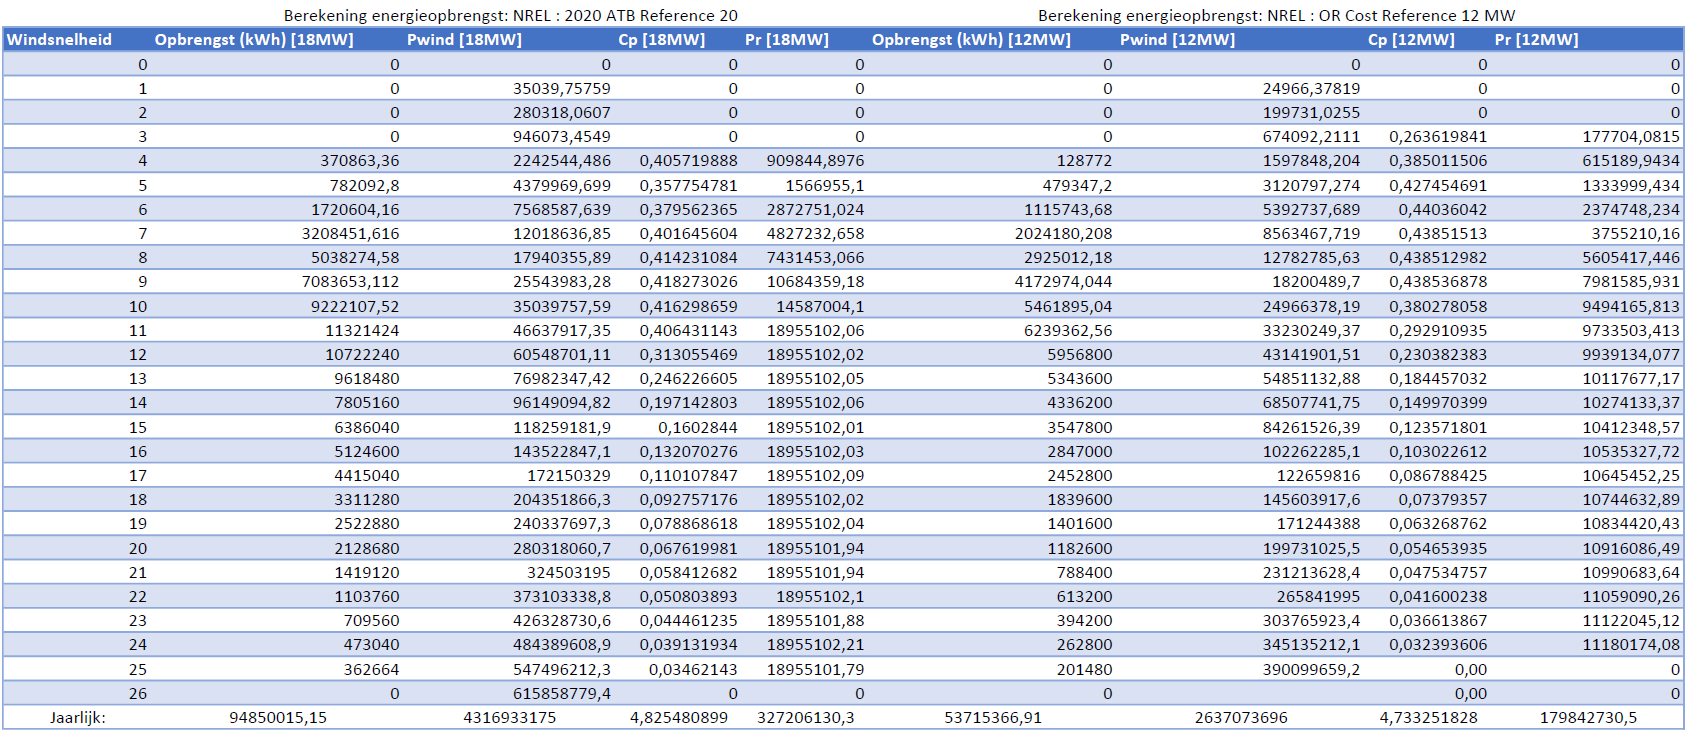
\includegraphics[width=1\textwidth]{IMG/data/overzicht/TVUW.PNG}
\caption{Gegevens: windsnelheid, energieopbrengst, vermogen en Cp}
\label{fig:TVUW}
\end{figure}

\subsubsection{Cp}
Elke windturbine heeft een vermogensfactor (Cp). Door het windvermogen te vermenigvuldigen met de Cp van de windturbine, wordt het werkelijk op te wekken vermogen verkregen. Ook de Cp is variabel, wat betekent dat het vermogen dat de turbine uit de wind kan halen ook zal verschillen afhankelijk van de windsnelheid. De plot van de Cp is te zien in (figuur \ref{fig:CpGraph}). De uitkomsten van de formules \ref{eq:5} en \ref{eq:6} zijn wederom genoteerd en geplot zoals te zien in (figuur \ref{fig:PrGraph}). 
\begin{figure}[H]
\centering
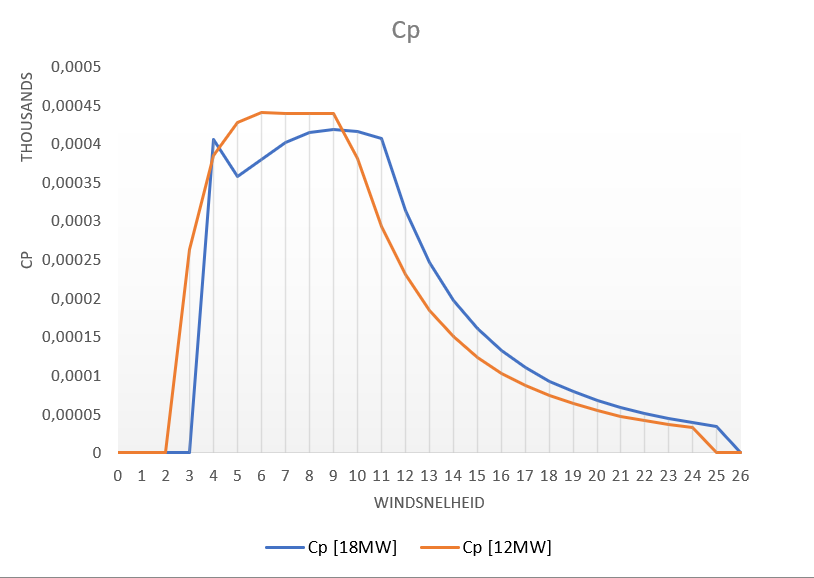
\includegraphics[width=0.7\textwidth]{IMG/data/overzicht/Cp_graph.PNG}
\caption{Plot: Cp\textsubscript{18MW} en Cp\textsubscript{12MW}}
\label{fig:CpGraph}
\end{figure}
\subsubsection{Pr}
\begin{figure}[H]
\centering
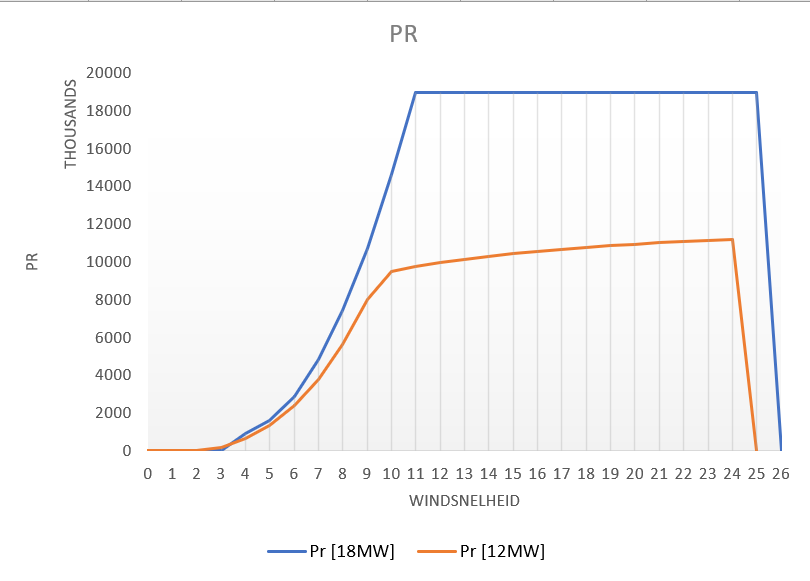
\includegraphics[width=0.7\textwidth]{IMG/data/overzicht/Pr_graph.PNG}
\caption{Plot: Pr\textsubscript{18MW} en Pr\textsubscript{12MW}}
\label{fig:PrGraph}
\end{figure}


\begin{equation} \label{eq:5}
\text{Werkelijk vermogen 12MW turbine: } P_{r12MW}=Cp_{12MW}*P_{wind12MW}
\end{equation}
\myequations{Berekening: Werkelijk vermogen 12MW turbine}

\begin{equation} \label{eq:6}
\text{Werkelijk vermogen 18MW turbine: } P_{r18MW}=Cp_{18MW}*P_{wind18MW}
\end{equation}
\myequations{Berekening: Werkelijk vermogen 18MW turbine}

\subsubsection{Wind data}
Uit de Wind Resource Assessment\cite{WindResourceAssessment} is de benodigde winddata gehaald. Hieronder valt ook informatie over de frequentie van gemeten windsnelheden gedurende een periode van twee jaar. Deze frequentie kan gebruikt worden als de kans op de windsnelheid. Met formule \ref{eq:7} kan berekend worden hoeveel uur een windsnelheid per jaar zal plaatsvinden als deze overeen komt met de bepaalde kans. In onderstaande formule (\ref{eq:7}) staat X voor de kans / het percentage dat de windsnelheid voorkomt in een jaar. 

\begin{equation} \label{eq:7}
\text{Frequentie windsnelheid in uren/jaar: } 365*24*X 
\end{equation}
\myequations{Berekening: Frequentie windsnelheid}


De verdeling van de frequentie van de windsnelheden over de span van de gemeten periode\cite{WindResourceAssessment} staat in (figuur \ref{fig:Frequentieverdeling}). 
\begin{figure}[H]
\centering
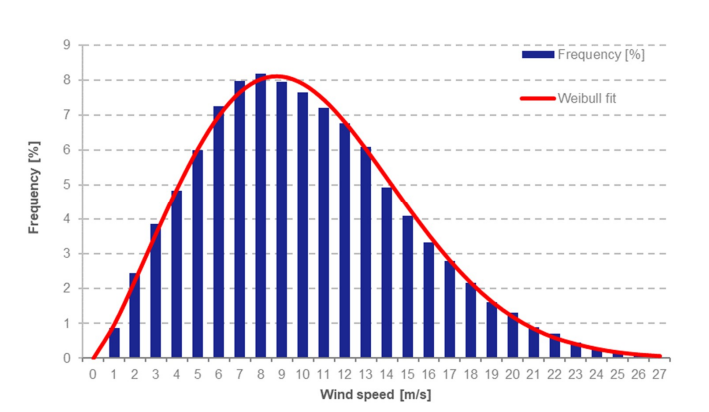
\includegraphics[width=0.7\textwidth]{IMG/data/overzicht/Frequentieverdelingwind.PNG}
\caption{Gegevens: frequentie wind snelheid per jaar.}
\label{fig:Frequentieverdeling}
\end{figure}

\subsubsection{Energieopbrengst exclusief parkeffect}
Door de verdeling van het aantal uur dat de windsnelheden voorkomen in een jaar en de berekende werkelijke vermogens van de windturbines te gebruiken, kan de jaarlijkse energieopbrengst worden berekend. Dit wordt gedaan met de volgende formules: 

\begin{equation} \label{eq:8}
\text{12MW Turbine: } E_{opbrengst,12MW}=t_{uren per jaar}*P_{r12MW}
\end{equation}
\myequations{Berekening: Energie Opbrengst 12MW Turbine}

\begin{equation} \label{eq:9}
\text{18MW Turbine: } E_{opbrengst,18MW}=t_{uren per jaar}*P_{r18MW}
\end{equation}
\myequations{Berekening: Energie Opbrengst 18MW Turbine}

De uitkomsten hiervan zijn in (tabel \ref{fig:Jaaropbrengst}) genoteerd. Nu kan de jaaropbrengst berekend worden voor beide turbines, door de uitkomsten van dezelfde turbine bij elkaar op te tellen. Hieruit is gekomen dat de jaaropbrengst met de 18MW turbine overeen komt met 94.850.015 kWh, en met de 12MW turbine overeen komt met 53.715.367 kWh. Dit verschil is behoorlijk en geeft duidelijk aan hoezo de 18MW windturbine veel voordeliger en aantrekkelijker is om te gebruiken. 
\begin{figure}[H]
\centering
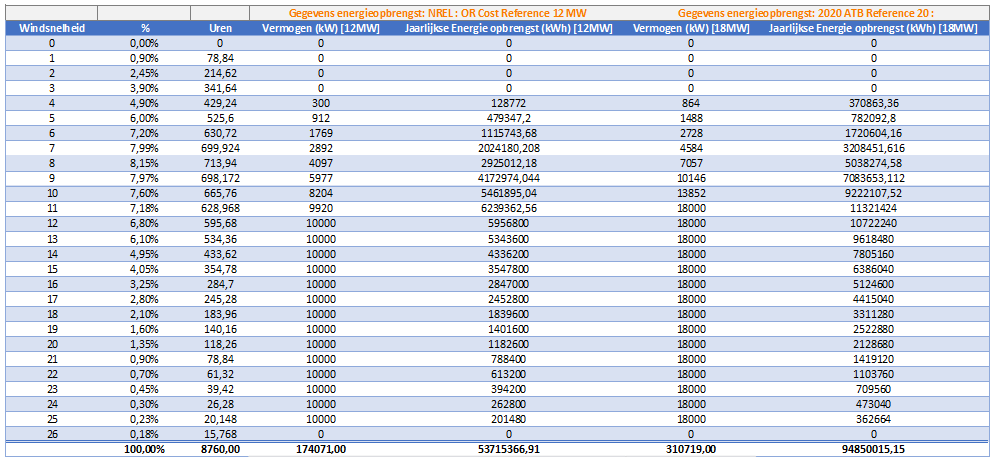
\includegraphics[width=1\textwidth]{IMG/data/overzicht/Jaaropbrengst.PNG}
\caption{Gegevens: Uren, Vermogens en Energieopbrengst.}
\label{fig:Jaaropbrengst}
\end{figure}
Bij deze jaarlijkse energieopbrengst is echter nog geen rekening gehouden met een aantal factoren die in de werkelijkheid een rol spelen, zoals het parkeffect. Om de jaarlijkse energieopbrengst inclusief het parkeffect te bepalen moet eerst het parkeffect berekend worden. Het parkeffect kan vervolgens vermenigvuldigd worden met de jaarlijkse energieopbrengst exclusief parkeffect, om de daadwerkelijke jaarlijkse energieopbrengst te krijgen. 

\subsubsection{Parkeffect}
Om dit parkeffect te berekenen, zijn een aantal tussenstappen gemaakt, waarbij verschillende berekeningen gemaakt zijn. De berekeningen moeten worden uitgevoerd voor beide kavels. Er is echter nog niet genoeg informatie gevonden over de oppervlaktes van de individuele kavels. Hier zal voor het volgende tussenrapportagemoment nog meer onderzoek naar gedaan worden. Voor nu is echter de oppervlakte van beide kavels bepaald door de oppervlakte van het windpark (176km\textsuperscript{2}) te delen door twee. Hierdoor is de oppervlakte voor beide kavels op het moment dus hetzelfde (88km\textsuperscript{2}), en verschilt er dus niks tussen de kavels. 

Om het parkeffect te berekenen zijn de volgende gegevens van belang: 
\begin{itemize}
    \item Aantal turbines per kavel
    \item Totale vermogen per kavel
    \item Oppervlakte kavel
    \item Vermogensdichtheid 
    \item Jaaropbrengst exclusief parkeffect
\end{itemize}

Ter vergelijking zijn deze berekeningen uitgevoerd voor beide windturbines. 

\subsection{Configuratie 1 (18MW)}
De eerste stap is het bepalen van het aantal turbines op de kavel. Volgens de eisen mag het totale rotoroppervlak niet groter zijn dan 2.624.613m\textsuperscript{2}, vanwege de grootte van het rotoroppervlak van de 18MW turbine, is de maximale hoeveelheid turbines die geplaatst kan worden volgens de eisen gelijk aan 48. 

De tweede stap is het totale vermogen op de kavel bepalen. Dit is het aantal turbines maal het vermogen per turbine, dus 48*18 = 864MW. Vervolgens moet de oppervlakte van het windpark bepaald worden. Hiervoor is, zoals eerder vermeld, dezelfde waarde genomen voor beide kavels, namelijk 88km\textsuperscript{2} wateroppervlak. 

Stap drie is het bepalen van de vermogensdichtheid. Om dit te berekenen kan de volgende formule gebruikt worden: 
\begin{equation} \label{eq:10}
\text{18MW Turbine: } P_{dichtheid18MW}=(\frac{n_{turbines}*P_{turbine}}{A_{oppervlak}}) = (\frac{48*18}{88}) = 9,818 MW/km\textsuperscript{2}
\end{equation}
\myequations{Berekening: P Dichtheid 18MW Turbine}

Vervolgens kan met de vermogensdichtheid het parkeffect berekend worden. Dit wordt gedaan met formule \ref{eq:11}. 

\begin{equation} \label{eq:11}
 Parkeffect_{18MW}=\frac{100-(\frac{n_{turbines}*P_{turbine}}{A})}{100} = \frac{100-P_{totaal}}{100}
\end{equation}
\myequations{Berekening: Parkeffect 18MW Turbine}

Het parkeffect varieert afhankelijk van de vermogensdichtheid. Deze is op zijn beurt weer afhankelijk van meerdere factoren. De berekende waardes van het parkeffect voor verschillende aantallen turbines staan in figuur \ref{fig:Parkeffect_table} is geplot in (figuur \ref{fig:ParkEffectGraph}). 

\begin{figure}[H]
\centering
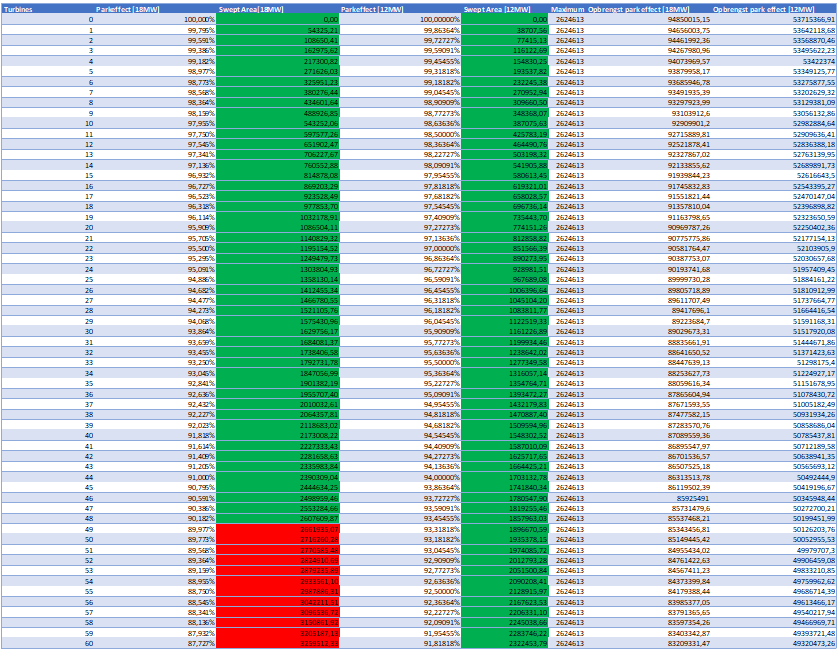
\includegraphics[width=1\textwidth]{IMG/data/overzicht/Parkeffect.PNG}
\caption{Gegevens: Aantal turbines, Parkeffect, Swept Area en Opbrengst park effect.}
\label{fig:Parkeffect_table}
\end{figure}

\begin{figure}[H]
\centering
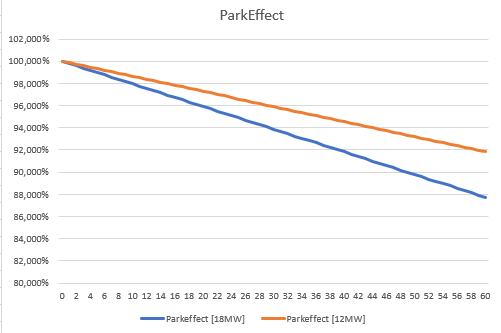
\includegraphics[width=0.7\textwidth]{IMG/data/overzicht/parkeffect_graph.PNG}
\caption{Plot: Parkeffect.}
\label{fig:ParkEffectGraph}
\end{figure}

Ten slotte kan met het parkeffect het daadwerklijke vermogen bepaald worden. Dit kan berekend worden door het parkeffect te berekenen voor het aantal turbines dat op de kavel komt. In dit geval gaat het om 48 turbines. Dus is het parkeffect: 

\begin{equation} \label{eq:12}
 Parkeffect_{18MW} = \frac{100-(P_{totaal}/A)}{100} = \frac{100-(864/88)}{100} = 0,902 = 90,2\%
\end{equation}
\myequations{Berekening: Parkeffect 18MW Turbine doorgerekend}

De jaarlijkse energieopbrengst inclusief het parkeffect is dan vrij simpel te berekenen met de formule: 
% \begin{equation} \label{eq:6}
% \text{Opbrengst 12MW kWh } t_{uren per jaar}*VermogenPerWindsnelheid_{12MW}
% \end{equation}
% \begin{equation} \label{eq:7}
% \text{Opbrengst 18MW kWh } t_{uren per jaar}*VermogenPerWindsnelheid_{18MW}
% \end{equation}


\begin{equation} \label{13}
\text{18MW Turbine: } OpbrengstParkeffect_{18MW}=Parkeffect_{18MW}*E_{opbrengst,18MW} 
\end{equation}
\myequations{Berekening: Opbrengst Parkeffect 18MW Turbine}

\begin{equation} \label{14}
OpbrengstParkeffect_{18MW}=0,902*94850015 = 85.554.713kWh 
\end{equation}
\myequations{Berekening: Opbrengst Parkeffect 18MW Turbine}

\subsection{Configuratie 2 (12MW)}
Voor configuratie 2 zijn de meeste berekeningen al uitgevoerd bij configuratie 1. Ook is het verschil duidelijk te zien in de figuren en is voor elke formule het alternatief gegeven voor de turbine van configuratie 2. 

De energieopbrengst inclusief parkeffect zal hieronder worden berekend voor de windturbine van 12MW. 

\begin{equation} \label{eq:15}
 Parkeffect_{12MW} = \frac{100-(P_{totaal}/A)}{100} = \frac{100-((60*12)/88)}{100} = 0,918 = 91,8\%
\end{equation}
\myequations{Berekening: Parkeffect 12MW Turbine doorgerekend}

\begin{equation} \label{eq:16}
OpbrengstParkeffect_{12MW}=Parkeffect_{12MW}*E_{opbrengst,12MW}
\end{equation}
\myequations{Berekening: Opbrengst Parkeffect 12MW Turbine}

\begin{equation} \label{eq:17}
OpbrengstParkeffect_{12MW}= 0,918*53715367 = 49.320.473 kWh
\end{equation}
\myequations{Berekening: Opbrengst Parkeffect 12MW Turbine}

Het verschil in jaarlijkse energieopbrengst, inclusief parkeffect, tussen de twee configuraties is dus 85.554.713 - 49.320.473 = 36.234.240 kWh aan energie per jaar. Dat is een zeer aanzienlijk getal. Dit is ook terug te zien in figuur \ref{fig:OpbrengstPark}

\begin{figure}[H]
\centering
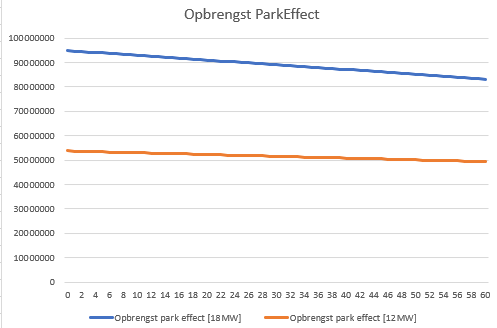
\includegraphics[width=0.7\textwidth]{IMG/data/overzicht/OpbrengstPark_graph.PNG}
\caption{Plot: OpbrengstPark.}
\label{fig:OpbrengstPark}
\end{figure}

% \section{Welke twee type windturbines zijn het meest geschikt voor het windpark en waarom?}
% Er zullen meerdere maatregelen worden genomen om de kwaliteit van de producten te waarborgen. Voor alle producten geldt dat er een eindredactie zal plaatsvinden. Bij de eindredactie zullen de documentaties worden gecontroleerd op inhoudelijke en verslagtechnische correctheid. Ook zullen voor alle producten alleen betrouwbare bronnen geraadpleegd worden met relevante informatie en actuele autoriteit. Daarnaast zal verwezen worden naar alle bronnen volgens de verslagtechnische eisen, met correcte toepassing van IEEE-richtlijnen. Verder zullen, ter verbetering van de leesbaarheid van het document, alle moeilijke termen genoteerd worden in een begrippenlijst.

% \subsection{Planning en taakverdelingen}
% Naast een eindredactie wordt, om de kwaliteit van de producten en de timing van de levering hiervan te garanderen, voor een goede organisatie gezorgd. Hieronder vallen een goede taakverdeling, planning en communicatie. Voor de taakverdeling en planning wordt het platform Github gebruikt, hierop zijn de taken per projectlid ingedeeld en ingepland. Zo kan worden verzekerd dat iedereen zich aan alle deadlines houdt. Als dit niet het geval blijkt te zijn, wordt dit besproken en zijn er consequenties. Naast Github is de planning ook in grote lijnen uitgewerkt in het plan van aanpak. 

% \subsection{Onderzoeksvragen}
% Met als doel het waarborgen van de structuur en kwaliteit van de documentaties, zal de probleemstelling worden opgedeeld in kleinere problemen. Deze problemen zullen worden uitgewerkt met behulp van onderzoeksvragen.\cite{projecthandleiding}
% De hoofdvraag voor het gehele project is: "\textbf{Hoe kunnen de eisen volgens het energieakkoord \cite{energieakkoord} van 2013 behaald worden met behulp van een windturbinepark op kavel VI en VII?}". De hoofdvraag zal worden beantwoord door middel van meerdere deelvragen. Voor tussenproduct 1, het park ontwerp, zullen de volgende vragen beantwoord worden\cite{projecthandleiding}:
% \begin{itemize}
%     \item Welke twee type windturbines zijn het meest geschikt voor het windpark en waarom?
%     \item Wat is de beste positionering van de windturbines voor optimale opbrengst, efficiënte bekabeling en makkelijker onderhoud?  
%     \item Welke kabels zijn geschikt voor het transporteren van de energie van turbines tot het hoogspanningsstation met de verwachte stromen?
%     \item Hoe ziet de bekabeling van het windpark eruit en waarom?
%     \item Wat  de beste soort spanning voor dit windturbinepark is, gelijk- of wisselspanning en welke effecten heeft dit op het park? %Bespreek transformator boxen
%     \item Welk invloed hebben de gemaakte keuzes op de onderhoud van het park? 
% \end{itemize}

% Ter beantwoording van tussenproduct 2, het onderhoudsplan, zijn de volgende deelvragen opgesteld:
% \begin{itemize}
%     \item Hoe wordt de conditie van de componenten waaruit het windturbinepark bestaat bewaakt? 
%     \item Welk onderhoud moet er plaatsvinden aan het windturbinepark?
%     \item Hoe frequent moet er onderhoud plaatsvinden en hoe is dit bepaald?
%     \item Hoe ziet de onderhoudsstrategie eruit? 
%     \item Welke materiële en financiële risico's zijn er bij het plegen van onderhoud?
% \end{itemize}

% Deze vragen uitgebreid beantwoorden garandeert dat alle belangrijke aspecten voor dit project behandeld worden. 

\section{Turbines}
\subsection{Introductie}
In de huidige wereld van hernieuwbare energie staan offshore windturbines als pion van een groenere toekomst. De keuze voor de juiste windturbine voor een project is cruciaal, en het verkrijgen van nauwkeurige en betrouwbare informatie over deze turbines is van het groot belang. Onderzoek heeft getoond dat er verscheidene turbines en fabrikanten zijn, waaronder de GE Haliade-X 14 MW, de Goldwind GWH252-16MW, de Vestas V236, de NREL 12MW en de NREL 18MW.
\subsection{GE Haliade-X 14 MW}
De GE Haliade-X 14 MW is een krachtige offshore windturbine met een aanzienlijk nominaal vermogen van 14 MW. Met een indrukwekkende rotordiameter van 220 meteren een jaarlijkse energieproductie van ongeveer 74 gigawattuur, speelt deze turbine een significante rol in de offshore windenergiesector. \cite{GEHalideX}\cite{TNOHalideX}\cite{TopsectorEnergieHalideX}\cite{OffshoreWindHalideX}\cite{AandrijftechniekHalideX}\cite{PonderaHalideX}
\subsection{Vestas V236}
De Vestas V236, met een vermogen van 15 MW en een rotordiameter van 236 meter, vertegenwoordigt eveneens een aanzienlijke keuze binnen de offshore windenergie sector. Desondanks wordt hij op het gebied van nominaal vermogen en jaarlijkse energieproductie overtroffen door de MySE-windturbine. \cite{Vestas15MW}\cite{Vestas}\cite{VestasJourney}\cite{WindTurbineModels}\cite{Electrek}\cite{OffshoreWindBiz3}
\subsection{Ming Yang MySE 16-260}
De MySE-windturbine, ontwikkeld door het Chinese bedrijf MingYang, heeft de aandacht getrokken vanwege zijn indrukwekkende technische specificaties en efficiëntie. Met een rotordiameter van 252 meter behoort deze windturbine tot de grootste in zijn categorie, wat hem in staat stelt om krachtige offshore winden effectief te benutten. Met een nominaal vermogen van 16 MW kan de MySE aanzienlijke hoeveelheden elektriciteit genereren, zelfs onder uitdagende omstandigheden.
Een opvallend kenmerk van de MySE-windturbine is zijn vermogen om windbronnen efficiënter te benutten dan sommige concurrenten. Dit wordt ondersteund door gegevens die aantonen dat de MySE vergelijkbare of zelfs grotere hoeveelheden elektriciteit kan produceren dan windturbines met een hoger nominaal vermogen.\cite{NewAtlas}\cite{MySEWebsite}\cite{OffshoreWindMySE}\cite{YouTube}\cite{MySEWebsite2}
\subsection{Goldwind GWH252-16MW}
De Goldwind GWH252-16MW, met een indrukwekkende rotordiameter van 252 meter, toont een opmerkelijke technologische prestatie. Echter, de beschikbare gegevens suggereren dat de MySE-windturbine van MingYang nog steeds vergelijkbare of zelfs grotere hoeveelheden elektriciteit kan genereren, wat impliceert dat de MySE mogelijk efficiënter is in het benutten van windenergiebronnen.\cite{Goldwind}\cite{4COffshore}
\subsection{National Renewable Energy Laboratory}
Na grondige overweging en uitgebreide vergelijkingen met deze concurrenten, is er besloten om de focus te richten op de windturbines van het National Renewable Energy Laboratory (NREL). En dat is om goede redenen.\cite{NRELVision}\cite{NRELAwards}
\subsubsection{NREL12MW}
De NREL 12MW Offshore windturbine, hoewel iets lager in vermogen dan zijn grotere broer, heeft ook indrukwekkende specificaties en prestaties. Met een rotordiameter van 222 meter en een geschatte jaarlijkse energieproductie van 12 gigawattuur, blijft deze windturbine een krachtige en efficiënte optie voor offshore windenergieprojecten.\cite{NRELOregonWindStudy}\cite{NRELATB2020}\cite{NRELReference12MW}\cite{NRELCsv12MW}

Specificaties van de NREL 12W Offshore windturbine:
\begin{itemize}
    \item \textbf{Naam:} NREL 12MW Offshore windturbine
    \item \textbf{Nominaal vermogen:} 12.000 kW
    \item \textbf{Geschatte windsnelheid:} 11 m/s
    \item \textbf{Aanvang windsnelheid:} 3 m/s
    \item \textbf{Stop windsnelheid:} 25 m/s
    \item \textbf{Rotordiameter:} 222 meter
    \item \textbf{Hubhoogte:} 136 meter
\end{itemize}


\subsubsection{NREL18MW}
Specificaties van de NREL 18MW Offshore windturbine:
\begin{itemize}
    \item \textbf{Naam:} NREL 18MW Offshore windturbine
    \item \textbf{Nominaal vermogen:} 18.000 kW
    \item \textbf{Geschatte windsnelheid:} 11 m/s
    \item \textbf{Aanvang windsnelheid:} 3 m/s
    \item \textbf{Stop windsnelheid:} 25 m/s
    \item \textbf{Rotordiameter:} 263 meter
    \item \textbf{Hubhoogte:} 150 meter
\end{itemize}

De NREL 18MW Offshore windturbine biedt enkele opmerkelijke voordelen die hem tot een uitstekende keuze maken. Met een nominaal vermogen van 18 MW, een indrukwekkende rotordiameter van 263 meter en een jaarlijkse energieproductie van maar liefst 80 gigawattuur, is deze windturbine een krachtige oplossing op zee. Zijn hoge capaciteitsfactor zorgt ervoor dat hij consistent een hoog rendement kan leveren en meer elektriciteit aan het net kan leveren.\cite{NRELReference18MW}\cite{NRELCSV18MW}\cite{NRELATB2020Specific}
\subsubsection{Vergelijking}
Bovendien bieden de NREL 18MW en NREL 12MW Offshore windturbines de geruststellende zekerheid van betrouwbare gegevens en informatie die online open source beschikbaar zijn. Om deze reden kan er een nauwkeurige berekeningen gemaakt worden en het project op de meest solide basis te bouwen.\cite{NRELTurbineModels}

De keuze voor de NREL 18MW en NREL 12MW Offshore windturbines is niet alleen gebaseerd op hun indrukwekkende technische specificaties, maar ook op de visie van het National Renewable Energy Laboratory om een schone energietoekomst voor de wereld te creëren. Hun inzet voor energiegerechtigheid en inclusieve ontwerpen sluit naadloos aan bij onze eigen waarden en doelen. \cite{NRELDiversity}\cite{NRELSustainability}\cite{NRELTurbineModels}
\subsection{Conclusie}
Terwijl de windturbines van MingYang, Goldwind en Vestas ongetwijfeld indrukwekkend zijn, hebben de NREL 18MW en NREL 12MW Offshore windturbines de overhand in termen van vermogen, efficiëntie en betrouwbare informatie. Het is een keuze die ons dichter bij een groenere, schonere toekomst brengt, waarin offshore windenergie een cruciale rol speelt in de transitie naar duurzame energiebronnen. Met de NREL 18MW en NREL 12MW Offshore windturbines aan onze zijde zijn we vastbesloten om een positieve impact te hebben op de wereld van hernieuwbare energie en een duurzamere planeet te creëren voor toekomstige generaties.
% \include{chapters/09_Wat is de beste positionering van de windturbines voor optimale opbrengst, efficiënte bekabeling en makkelijker onderhoud?}
% \section{Risico’s}
Het ontwerpen van een windturbinepark en het opstellen van een onderhoudsplan zijn complexe projecten waarbij verschillende interne en externe risico's kunnen optreden. De risico´s kunnen verschillen van tijdsgebonden problemen tot technische complicaties. 

Het niet volledig begrijpen van de doelstellingen en eisen van het project, en/of onvoldoende communicatie tussen teamleden, belanghebbenden en experts kan resulteren in misverstanden, vertragingen, onsamenhangende of niet relevante informatie en overige fouten in de documenten. Daarom is, om dit te voorkomen, vooraf het plan van aanpak opgesteld. Daarnaast zal aan het begin van het project een analysefase plaatsvinden waarin de doelstellingen duidelijk worden voor de projectleden. Verder wordt er iedere week gecommuniceerd tussen de projectleden en worden wijzigingen in Github genoteerd. Zo wordt ervoor gezorgd dat op dit front niks fout gaat. 

Gebrek aan kennis kan ook zorgen voor problemen. Het projectteam heeft mogelijk onvoldoende kennis of ervaring met windturbineparkontwerp en -onderhoud, wat kan leiden tot onjuiste aanbevelingen. Het is daarom van belang dat het projectteam genoeg onderzoek doet en hun kennis uitbreid gedurende het project. Als het niet lukt de benodigde informatie te vinden of kennis op te doen, zal er naar alternatieve externen moeten worden gezocht voor hulp. Dit zal ervoor zorgen dat gebrek aan kennis geen barricade zal vormen, de teamleden hun kennis uitbreiden en toepassen om zo toch correcte en goede kwaliteit producten te kunnen leveren. 

Tijdsgebrek is ook een risico. Tijdsdruk om het parkontwerp en onderhoudsplan binnen strakke deadlines op te stellen, kan leiden tot gehaaste beslissingen en onvolledigheid van de documenten. Door goed te plannen en voor te bereiden zal dit worden voorkomen. 

Technologische veranderingen kunnen goed zijn, echter kan het ook voor problemen zorgen. Snelle technologische vooruitgang kan van invloed zijn op de keuze van apparatuur en systemen in het ontwerp en het onderhoudsplan, wat herziening noodzakelijk kan maken. Dit is een risico dat niet voorkomen kan worden. Het effect kan echter wel beperkt worden door op een bepaald moment een definitief besluit te nemen over de apparatuur en systemen die gebruikt zullen worden. 

Ten slotte zijn er nog financiële risico's. Beperkt budget kan de mogelijkheden limiteren. Daarnaast kunnen verschillende onverwachte gebeurtenissen gedurende het project zorgen voor verhoogde kosten. Mocht dit voorkomen, dan zal de situatie met de opdrachtgever besproken worden en zal gezocht worden naar een oplossing.
% \section{Verdeling van hoofdstukken}
 % Please add the following required packages to your document preamble:
% \usepackage[table,xcdraw]{xcolor}
% If you use beamer only pass "xcolor=table" option, i.e. \documentclass[xcolor=table]{beamer}
\begin{table}[h]
\begin{tabular}{|r|l|}
\hline
\rowcolor[HTML]{9B9B9B} 
\multicolumn{1}{|c|}{\cellcolor[HTML]{9B9B9B}\textit{\textbf{Hoofdstuk}}} & \multicolumn{1}{c|}{\cellcolor[HTML]{9B9B9B}\textit{\textbf{Teamlid}}} \\ \hline
\rowcolor[HTML]{EFEFEF} 
1 & Francisco Ramirez Ramirez \\ \hline
2 & Laurens van der Drift \\ \hline
\rowcolor[HTML]{EFEFEF} 
3 & Tommy Dobos \\ \hline
4 & Justin van der Reijden \\ \hline
\rowcolor[HTML]{EFEFEF} 
5 & Laurens van der Drift \\ \hline
6 & Tommy Dobos \\ \hline
\rowcolor[HTML]{EFEFEF} 
7 & Francisco Ramirez Ramirez \\ \hline
8 & Justin van der Reijden \\ \hline
\rowcolor[HTML]{EFEFEF} 
9 & Francisco Ramirez Ramirez \\ \hline
10 & Justin van der Reijden \\ \hline
\rowcolor [HTML]{EFEFEF}
Eindredactie & Tommy Dobos \\ \hline
\end{tabular}
\end{table}
% \section{Verdeling van hoofdstukken}
 % Please add the following required packages to your document preamble:
% \usepackage[table,xcdraw]{xcolor}
% If you use beamer only pass "xcolor=table" option, i.e. \documentclass[xcolor=table]{beamer}
\begin{table}[h]
\begin{tabular}{|r|l|}
\hline
\rowcolor[HTML]{9B9B9B} 
\multicolumn{1}{|c|}{\cellcolor[HTML]{9B9B9B}\textit{\textbf{Hoofdstuk}}} & \multicolumn{1}{c|}{\cellcolor[HTML]{9B9B9B}\textit{\textbf{Teamlid}}} \\ \hline
\rowcolor[HTML]{EFEFEF} 
1 & Francisco Ramirez Ramirez \\ \hline
2 & Laurens van der Drift \\ \hline
\rowcolor[HTML]{EFEFEF} 
3 & Tommy Dobos \\ \hline
4 & Justin van der Reijden \\ \hline
\rowcolor[HTML]{EFEFEF} 
5 & Laurens van der Drift \\ \hline
6 & Tommy Dobos \\ \hline
\rowcolor[HTML]{EFEFEF} 
7 & Francisco Ramirez Ramirez \\ \hline
8 & Justin van der Reijden \\ \hline
\rowcolor[HTML]{EFEFEF} 
9 & Francisco Ramirez Ramirez \\ \hline
10 & Justin van der Reijden \\ \hline
\rowcolor [HTML]{EFEFEF}
Eindredactie & Tommy Dobos \\ \hline
\end{tabular}
\end{table}
\phantomsection
\addcontentsline{toc}{section}{Referenties}
\printbibliography
\end{document}
